% Chapter 4
\chapter{Results of Calibration and 3D Reconstruction} % Main chapter title
\label{chapterCaliResultsReconstruction} % For referencing the chapter elsewhere, use \ref{sens_CalibrationSystem} 
%
\begin{figure}[!b]
\hspace*{-0.3cm}
\centering
\subfloat[Image Space][Image Space]{
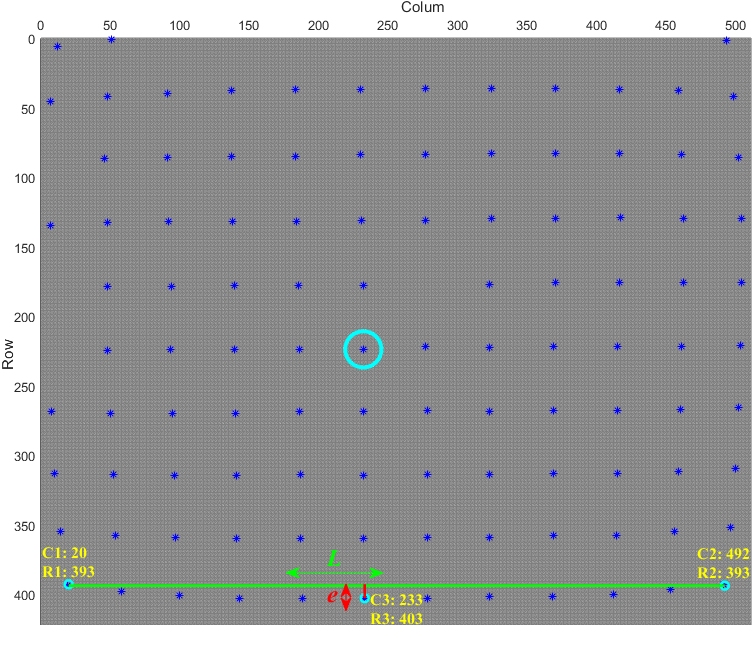
\includegraphics[width=0.5\textwidth]{Original_MatlabPrototype}
\label{Original_MatlabPrototype}}
%\qquad
\subfloat[\(1^{st}\) Order][\(1^{st}\) Order]{
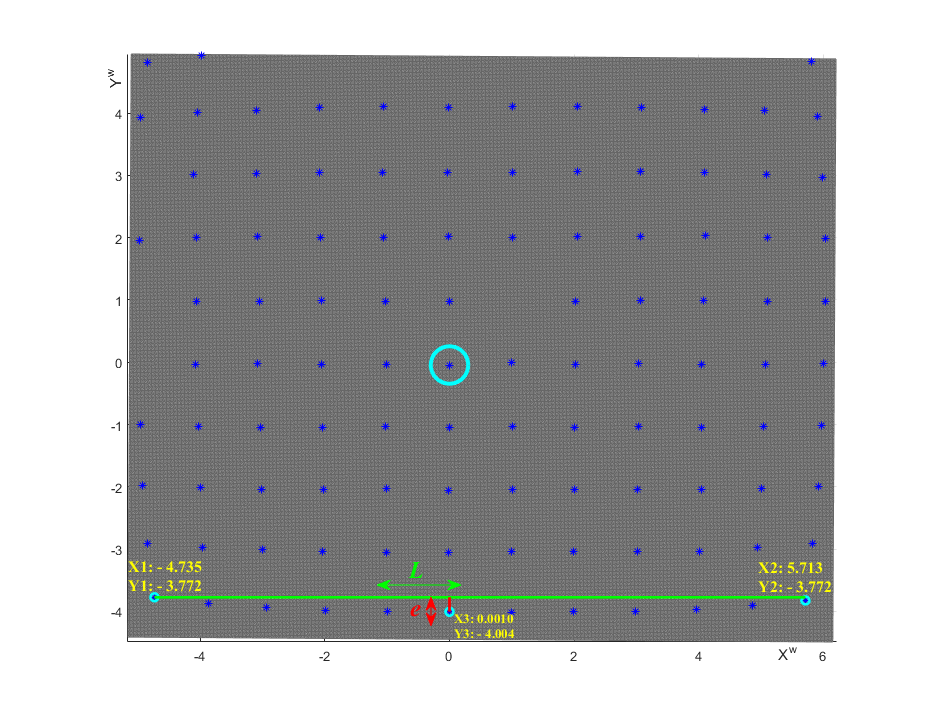
\includegraphics[width = 0.5\textwidth]{First_MatlabPrototype}
\label{First_MatlabPrototype}}

\subfloat[\(2^{nd}\) Order][\(2^{nd}\) Order]{
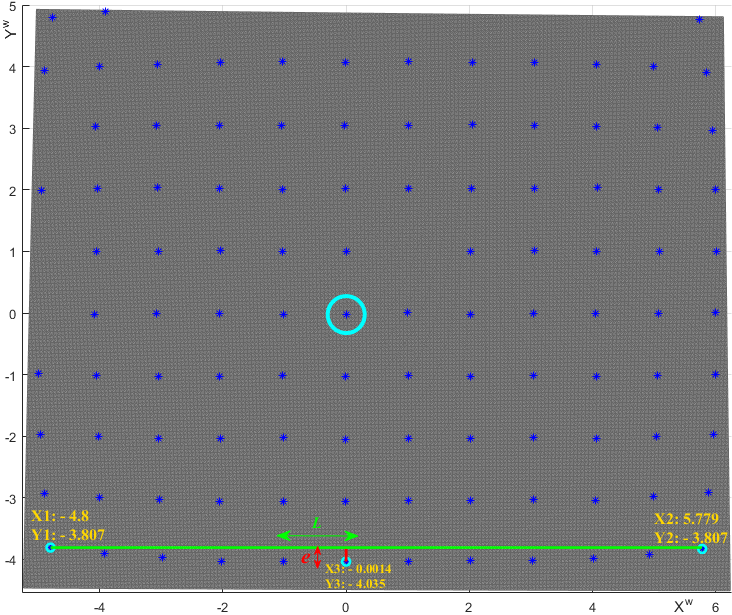
\includegraphics[width=0.5\textwidth]{Second_MatlabPrototype}
\label{Second_MatlabPrototype}}
%\qquad
\subfloat[\(4^{th}\) Order][\(4^{th}\) Order]{
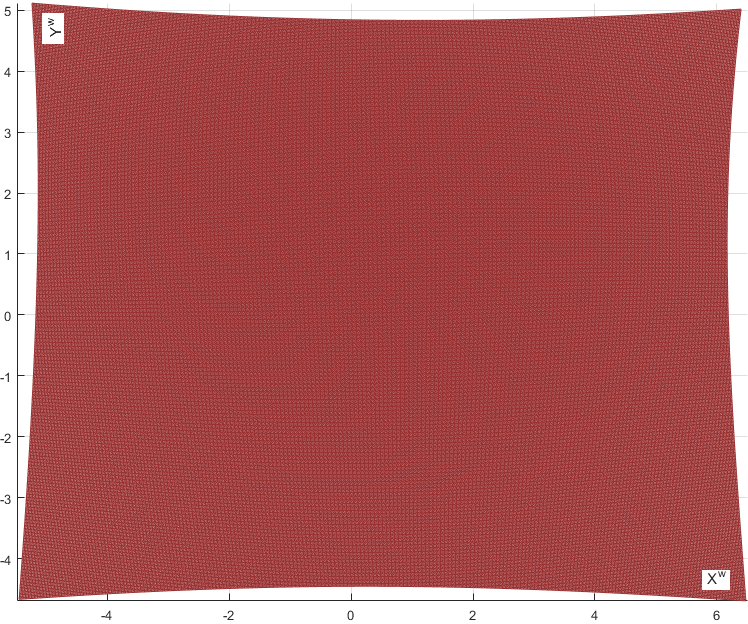
\includegraphics[width = 0.5\textwidth]{Fourth_MatlabPrototype}
\label{Fourth_MatlabPrototype}}
%
\caption{\(X^W\)\(Y^W\) Matlab Polynomial Prototype}
\label{MatlabPrototpyeOfHighOrder}
\end{figure}%
%
%%
\section{Calibration Results}
\label{sectionPrototypeTwoDtransformation} 
As discussed in section~\ref{perpixelDataCollection}, the per-pixel calibration method requires a two-dimensional high-order polynomial model to remove lens distortions and generate estimated (\(X^W,\, Y^W\))s from image space (\(R, \, C\))s. In this section, we will show detailed comparisons among different order polynomial results of both Matlab prototypes and real-time live applications. Figure~\ref{MatlabPrototpyeOfHighOrder} shows the Matlab prototypes of the simulated original image, world space \(X^WY^W\) plane result after a two-dimensional \(1^{st}\) order polynomial transformation, \(2^{nd}\) order polynomial and \(4^{th}\) order polynomial transformation. %
%
\\\indent
With squared-shaped distributed points (\(C,\, R\))s extracted from image streams, we can recover the original distorted image in Matlab, as shown in fig.\ref{Original_MatlabPrototype}. Using a mathematical distortion (\(d\)) measurement \cite{distortionMeasurement_2012}
%
\begin{equation}
d (\%)=  e*100/L ,
\label{mathematicalDistortion}
\end{equation}%
%
\noindent
we can get the original distortion \(d_0 = (R3 - R1) / (C2 -C1) = (403 - 393) / (492 - 20) = 2.1\%\). Fig.~\ref{First_MatlabPrototype} shows estimated world space \(X^WY^W\) plane after a two-dimensional \(1^st\) order polynomial transformation, whose distortion \(d_1 = (Y1 - Y3) / (X2 -X1) = [-3.772 - (-4.004)] / [5.713 - (-4.735)] = 2.2\%\). As we may have expected, the distortion \(d_1\) is not getting smaller at all. Fig.~\ref{Second_MatlabPrototype} and fig.~\ref{Fourth_MatlabPrototype} show the transformed world space \(X^WY^W\) plane images after the \(2^{nd}\) order and \(4^{th}\) order polynomial transformation respectively, from which we can get \(d_2 = [-3.807 - (-4.035)] / [5.779 - (-4.8)] = 2.1\%\) and \(d_4 = [-3.936 - (-3.992)] / [5.923 - (-4.928)] = 0.516\%\). It is straightforward to tell that, \(d_4\) is much smaller than \(d_0\) and fig.~\ref{Fourth_MatlabPrototype} intuitively shows a satisfying undistorted image. From eqn.~\ref{secondOrderPolynomial} and eqn.~\ref{fourthOrderPolynomial}, we know that the second order polynomial mapping has 2x6=12 parameters, and the fourth order polynomial mapping has 2x15=30 parameters. The higher order polynomial we use, the better radial distortion we are able to correct. In the meantime, the distortion removal model will have more parameters to calculate, and need more calibrating points to train the model.%
%
\\\indent
\begin{figure}[!t]
\centering
\hspace*{-0.3cm}
\subfloat[Before transformation][Before transformation]{
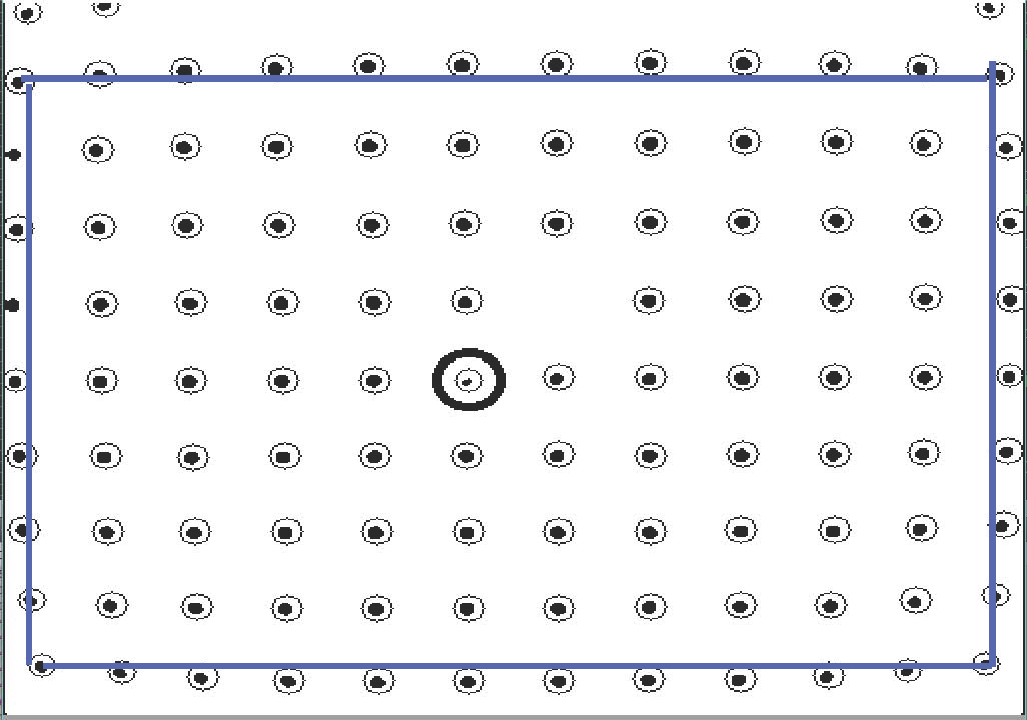
\includegraphics[width=0.5\textwidth, height = 0.425\textwidth]{BeforeRectification_Single_NIR}
\label{BeforeRectification_Single_NIR}}
%
\subfloat[Perspective Correction][Perspective (\(1^{st}\))]{
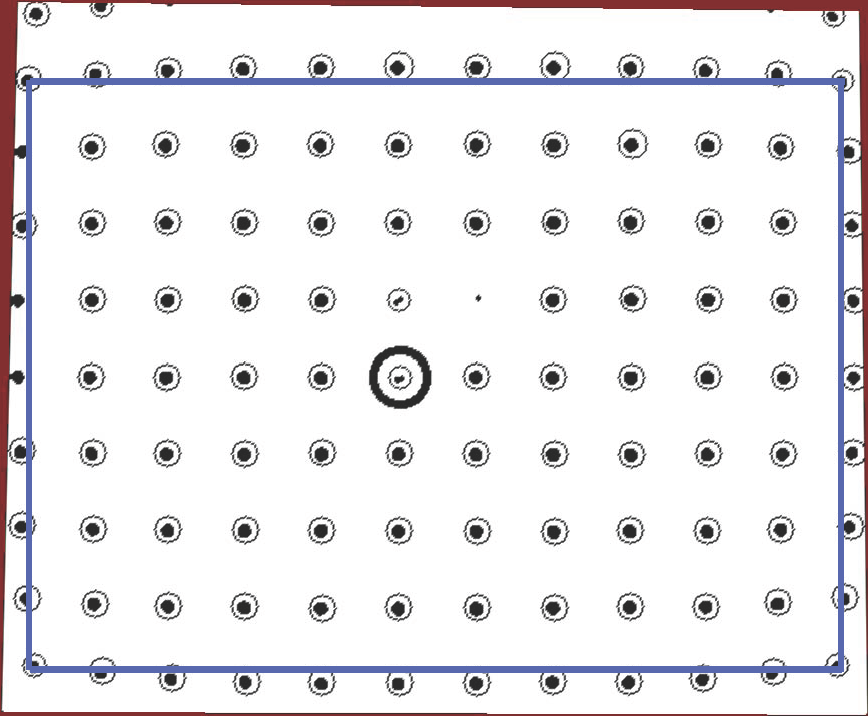
\includegraphics[width = 0.5\textwidth, height = 0.425\textwidth]{Perspective_QtScreenShot}
\label{Perspective_QtScreenShot}}
%
\\%\qquad
\hspace*{-0.3cm}
\subfloat[\(2^{nd}\) Order][\(2^{nd}\) Order]{
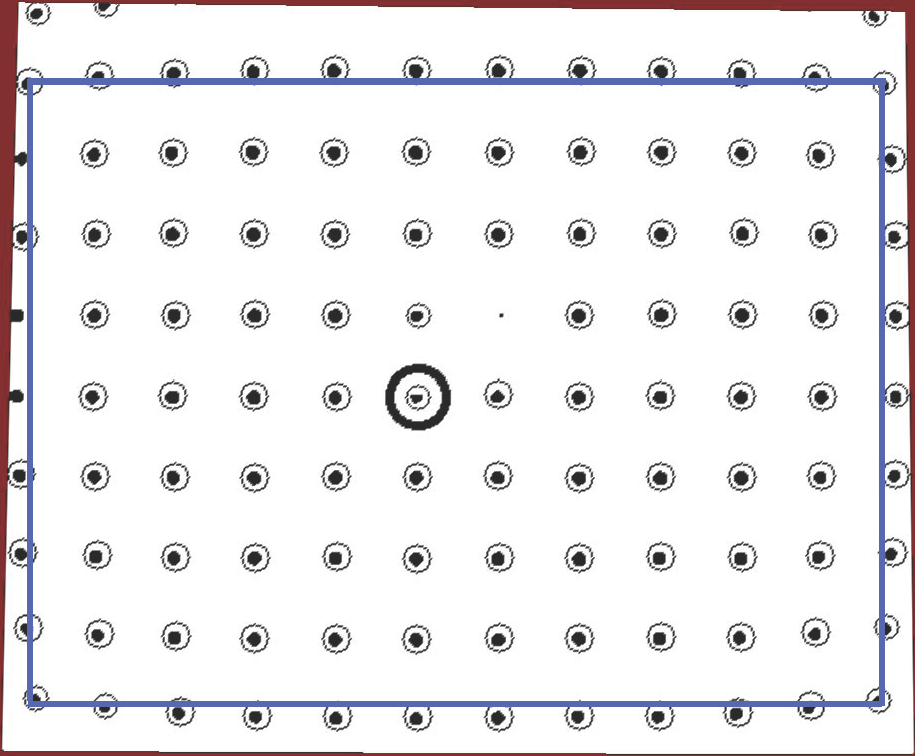
\includegraphics[width = 0.5\textwidth, height = 0.425\textwidth]{Second_QtScreenShot}
\label{Second_QtScreenShot}}
%
\subfloat[\(4^{th}\) Order][\(4^{th}\) Order]{
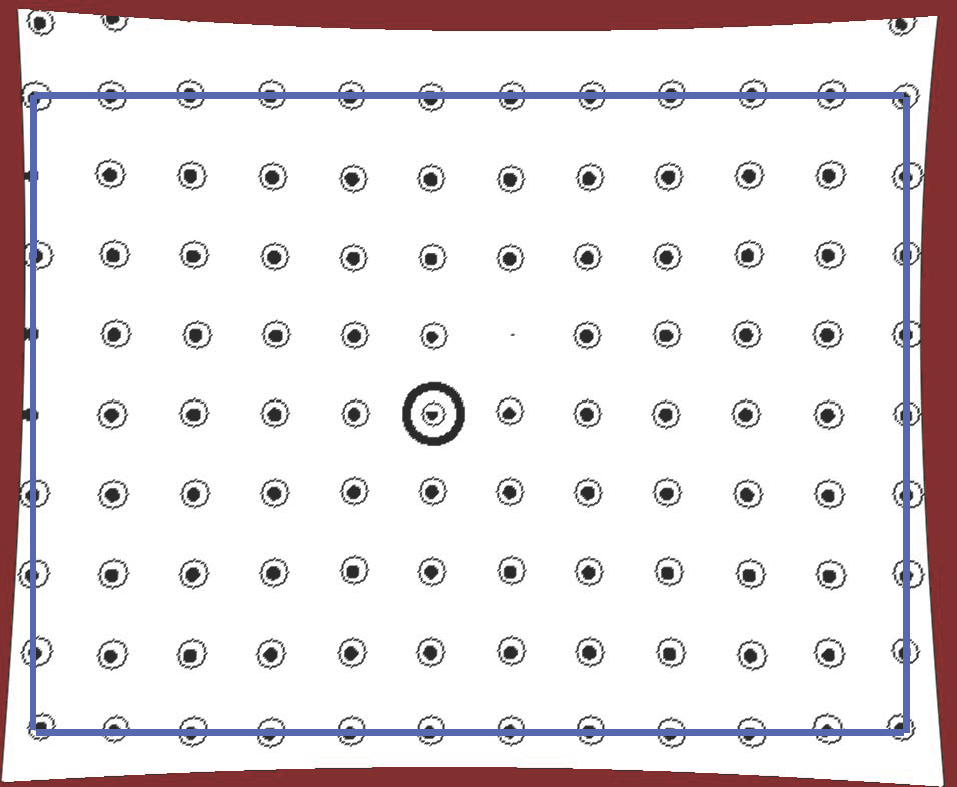
\includegraphics[width = 0.5\textwidth, height = 0.425\textwidth]{Fourth_QtScreenShot}
\label{Fourth_QtScreenShot}}
%
\caption{NearIR Stream High Order Polynomial Transformation}
\label{HighOrderNearIRRectification}
\end{figure}%
%
By applying those two-dimensional polynomial models into real-time streams transformation, we can get the transformed stream images. As shown in fig.~\ref{HighOrderNearIRRectification}, the outlines of the transformed steam images are same with Matlab prototypes in fig.~\ref{MatlabPrototpyeOfHighOrder}. It is easy to tell that the \(4^{th}\) order polynomial surface mapping is much better than the second order, and a higher order than \(4^{th}\) should be more accurate. However, as the order of the polynomial mapping goes higher, the number of parameters also get larger and larger, which costs more calculations and requires more data (coordinate-pairs) for training the transformation model. Considering that a \(5^{th}\) order polynomial mapping will have much more  parameters (2x21=42) to calculate while may not enhance much accuracy, we choose the \(4^{th}\) order polynomial as the main mapping model to get \(X^WY^W\) values from \(RC\). Limited by the static dot pattern, fewer and fewer dot-clusters could be observed by the camera as the camera getting closer to the dot pattern. Practically, \(4^{th}\) order calibration is replaced by \(2^{nd}\) order to guarantee a robust software when the observed dot-clusters are too few to train the transformation model.
\\\indent
%%
%%
%% %% mapping model parameters determination
%
\begin{figure}[t]
\centering
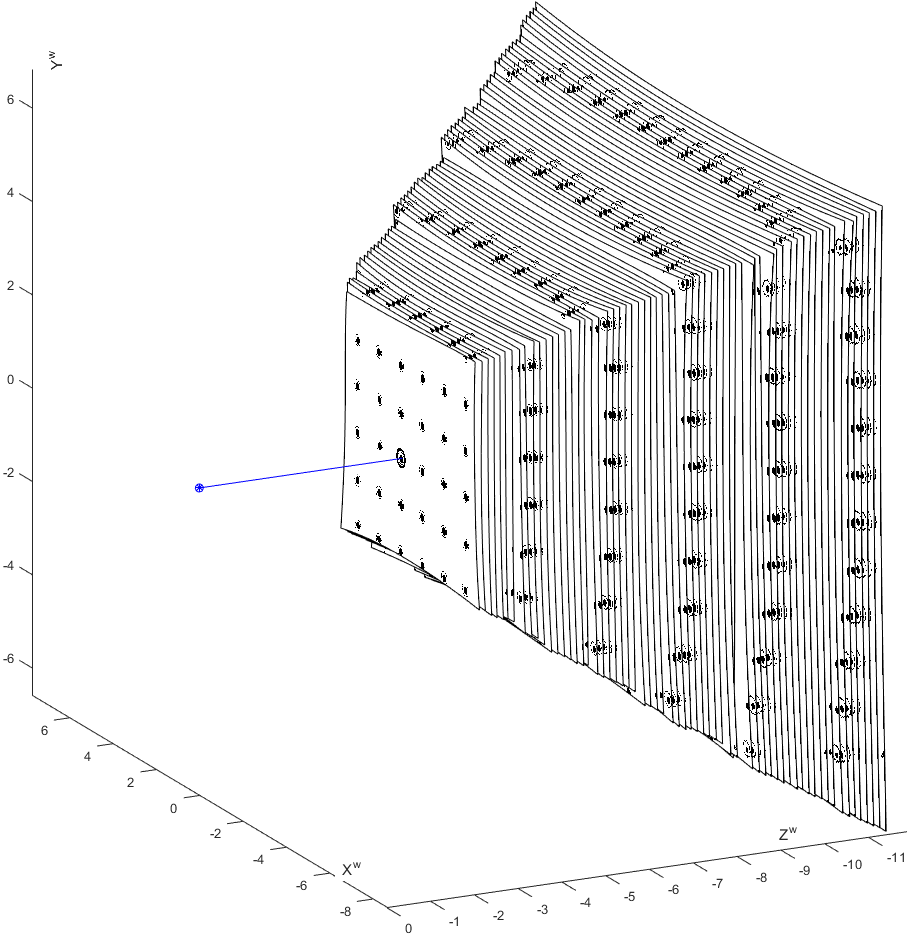
\includegraphics[width=0.7\textwidth, height= 0.55\textwidth]{Data63FranesForLUT}
\caption{63 Frames NearIR Calibrated 3D Reconstruction}
\label{Data63FranesForLUT}
\end{figure}%
%
%
\begin{figure}[t]
\centering
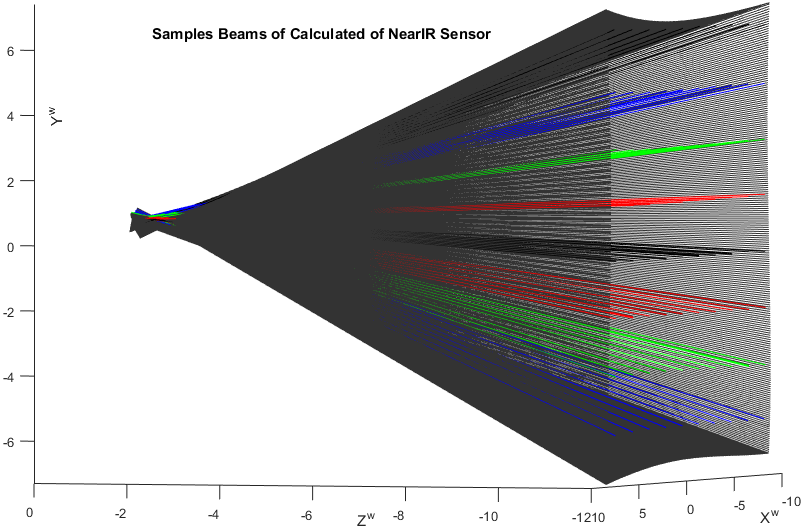
\includegraphics[width=0.6\textwidth]{SampleBeams_NearIR}
\caption{Sample Beams of Calibrated NearIR Field of View}
\label{SampleBeams_NearIR}
\end{figure}
%
The two-dimensional high-order polynomial mapping model will be applied in the first calibration step of \(X^\text{W}Y^\text{W}Z^\text{W}+D\) frames data collection. Figure~\ref{Data63FranesForLUT} shows 63 frames of collected \(X^\text{W}Y^\text{W}Z^\text{W}\), which gives an pyramid shape of a camera sensor's undistorted world space field of view. For each single pixel, its field of view is a beam, which could be mathematically expressed as equation.~\ref{kaiBeamEquationCh3}. Some sample beams are shown in fig.~\ref{SampleBeams_NearIR}, whose beam equation parameters \(c\)/\(d\)/\(e\)/\(f\) are determined as the best-fit totally by the collected undistorted data. 

\clearpage
%%%%%%%%%%%%%%%%%%%%%%%%%%%%%%%%%%%%%%%%%%%%%%%%%%%%%%%%%%%%%%%%%%%%%%%%%%%%%%%%%%%%%%%%%%%%%%%%%%%%%%%%%%%%%%%%%%%%%%%%%%%%%%%%%%%%%%%%%%%%%%%%%%%%%%%%%%%%%%%%%%%%%%%%%%%%%%%%%%%%%%%%%%%%%%%%%%%%%%%%%%%%%%%%%%%%%%%%%%%%%%%%%%%%%%%%%%%%%%%%%%%%%%%%%%%%%%%%%%%%%%%%%%%%%%

\section{Real-Time 3D Reconstruction on GPU}
%
\begin{figure}[b]
\centering
\hspace*{-0.3cm}
\subfloat[Raw (Distorted)]{
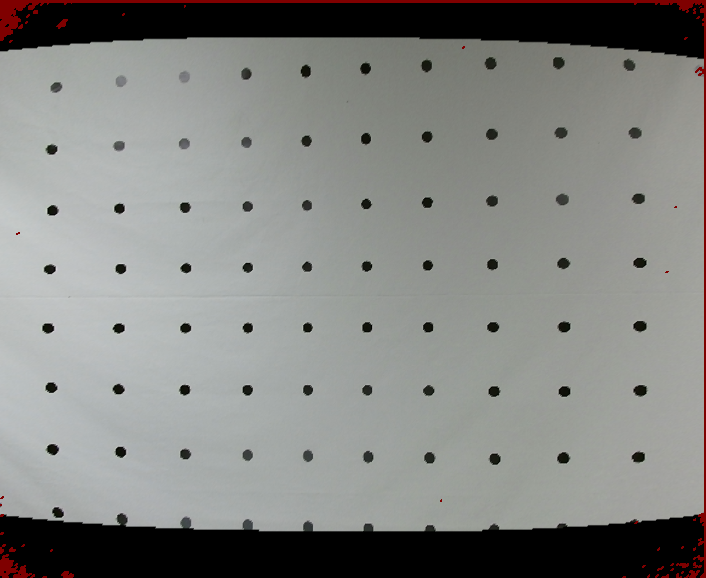
\includegraphics[width=0.5\textwidth, height = 0.425\textwidth]{distortedRGB}
\label{distortedRGB}}
%
\subfloat[Calibrated]{
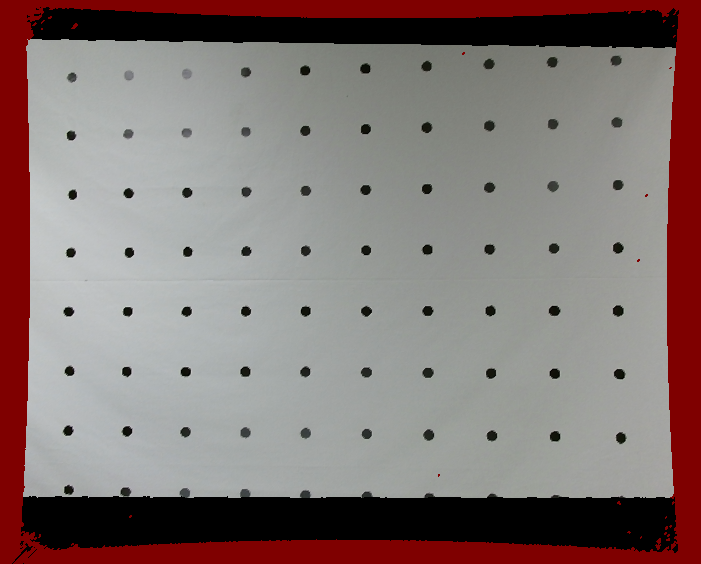
\includegraphics[width = 0.5\textwidth, height = 0.425\textwidth]{CalibratedRGB}
\label{CalibratedRGB}}
%
\caption{Lens-Distortions Removal by Per-Pixel Calibration Method}
\label{perPixelCalibrationBeforeAfter}
\end{figure}%
%
The 3D Reconstruction of undistorted \(X^\text{W}/Y^\text{W}/Z^\text{W}\) in real-time is the final aim of a 3D camera's calibration. In the traditional camera calibration method, which consist of one pinhole-camera matrix to generate raw world space 3D coordinates and another model for lens distortion removal, three big transformations are needed to generate the world space coordinates: from 2D distorted image space to 2D undistorted image space, then to 3D camera space, and finally to 3D world space. For every single pixel's processing, it needs 5 parameters from distortion removal model for the first step non-linear calculation, and then a 3x3 intrinsic matrix to get its camera space coordinates, and a 3x4 extrinsic matrix to finally acquire the world space coordinates. The 3D reconstruction after the traditional calibration requires a lot of calculations for every single pixel, and \emph{depth distortion} is not corrected at all.
\\\indent
\begin{figure}[t]
\centering
\hspace*{-0.3cm}
\subfloat[Raw]{
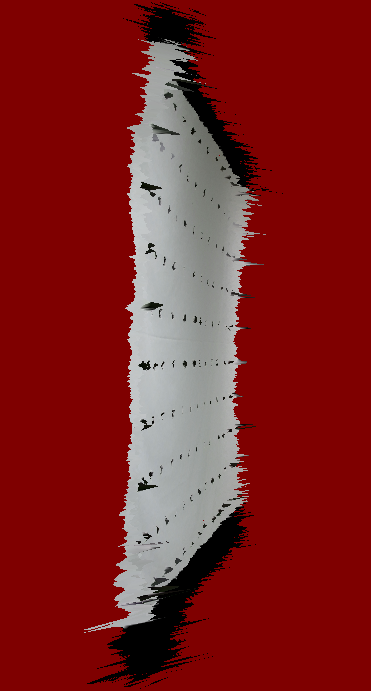
\includegraphics[width=0.3\textwidth, height = 0.425\textwidth]{distortedSideViewRGB}
\label{distortedSideViewRGB}}
\qquad%
\subfloat[Calibrated]{
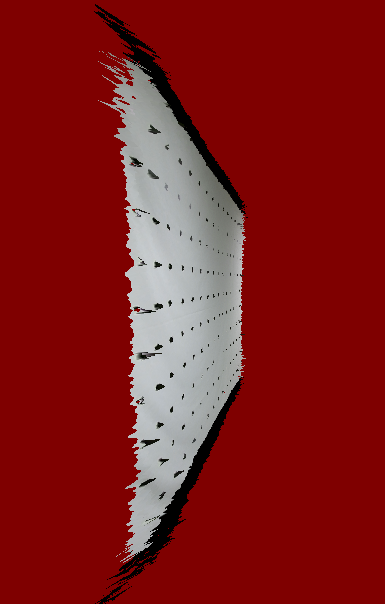
\includegraphics[width = 0.3\textwidth, height = 0.425\textwidth]{CalibratedSideView}
\label{CalibratedSideView}}
%
\caption{Depth-Distortions Removal by Per-Pixel Calibration Method}
\label{depthDistortionCalibrationBeforeAfter}
\end{figure}%
%
Using the proposed per-pixel calibration method, only three linear calculations with six parameters are needed to determine the world space coordinates for every single pixel. Two parameters \(e/f\) are utilized to generate world space \(Z^W\), as expressed in eqn.~(\ref{fromD_To_Z}). And the other four parameters \(a/b/c/d\) are applied to get \(X^W/Y^W\) respectively based on eqn.~(\ref{kaiBeamEquationCh3}). In this way, there is no need to calculate any non-linear equation for distortions removal, and the camera space is totally left aside. Combining two equations together, the undistorted 3D world coordinates (\(X^\text{W}, \, Y^\text{W}, \, Z^\text{W}\)) for every single pixel could be looked up based on \(D\) from a \(column\)-by-\(row\)-by-\(6\) look-up table. Figure~\ref{perPixelCalibrationBeforeAfter} shows how lens distortions are moved, and fig.~\ref{depthDistortionCalibrationBeforeAfter} shows how the \emph{depth distortion} is removed by per-pixel \(D\) to \(Z^W\) mapping.
%
%
%

















